%*************************************************************************************************************
% PREAMBLE STUFF
%*************************************************************************************************************
% Instead of inserting my \usepackage and defined commands here, I keep them in a separate file
\include{myPreamble}

%*************************************************************************************************************
% INCLUDE ONLY
%*************************************************************************************************************
% Use if you want to include only certain parts of the document, example \includeonly{introduction}
% in order to speed up compile time when you're focussing on some particular part.
%\includeonly{}

%*************************************************************************************************************
% DOCUMENT
%*************************************************************************************************************

\begin{document}

%*************************************************************************************************************
% TITLE
%*************************************************************************************************************

\title{Thesis Title\\[1ex]Second Line if Necessary}

\author{Author Name}

\dept{School of Computing}
\degree{Master of Science}

% OPTIONAL HERE
% ~~~~~~~~~~~~~
% \submitdate{month year in which submitted to GPO}
%        - date LaTeX'd if omitted
% \copyrightyear{ear degree conferred}
%        - year LaTeX'd if omitted
% \figurespagetrue or \figurespagefalse
%        - produce or don't produce a List of Figures page (true by default)
% \tablespagetrue or \tablespagefalse
%        - produce or don't produce a List of Tables page (true by default)

\beforepreface

% Adding single spacing so abstract and table of contents is single spaced.

%*************************************************************************************************************
% ABSTRACT
%*************************************************************************************************************

\prefacesection{Abstract}

The advent of social media has enabled political parties to engage with the
broader populous in new and unforeseen ways. This, coupled with rising levels of
political polarization has prompted debates as to whether people care about
policy anymore, or if they self-select into political bubbles online based on
their chosen party leader. This thesis proposes a novel adaptation of stochastic
blockmodelling to measure the degree to which political engagement on Twitter
was driven by policy or party leaders. Building on a graph theoretical approach,
measures of topic centrality are developed to give a measurement for how
efficient topics were at either spanning party leaders' bases, or appealing to
them. This is done in the context of Canada's 2019 federal election.


%*************************************************************************************************************
% CO-AUTHORSHIP (if necessary)
%*************************************************************************************************************

%\prefacesection{Co-Authorship}

%*************************************************************************************************************
% ACKNOWLEDGEMENTS
%*************************************************************************************************************

\prefacesection{Acknowledgments}

Blah blah blah.

%*************************************************************************************************************
% STATEMENT OF ORIGINALITY (required CHEM, CISC, GEOL, MATH, PHYS (Ph.D. only))
%*************************************************************************************************************

\prefacesection{Statement of Originality}

Only required by CHEM, COMPUTING, GEOL, MATH and Physics (Ph.D. ONLY!).


\singlespacing \afterpreface \doublespacing

%*************************************************************************************************************
% MEATY CHAPTERS
%*************************************************************************************************************

%Testing my index\index{index} abilities.  And
%sub-entry\index{index!subentry} abilities.

% This command can be used to view the page layout for this document
% \layout

% Here, I'm tweaking how much space is put above and below floats.
% Comment out if you want the *purest* latex spacing.
%\setlength{\abovedisplayskip}{3pt plus1pt minus1pt}
%\setlength{\abovedisplayshortskip}{3pt plus1pt minus1pt}
%\setlength{\belowdisplayskip}{3pt plus1pt minus1pt}
%\setlength{\belowdisplayshortskip}{3pt plus1pt minus1pt}


% Include my chapter texts - kept separated to make editing easier.
%


\newglossaryentry{UML}
{name=UML,
 description = {The Unified Modeling Language is a language ... ~\cite{Flo02}}
}



\chapter{Introduction}

\section{Background}

The advent of social media has enabled political parties to engage with the
broader populous in new and unforeseen ways. The ability to bypass the
traditional mediating forces of mass media allows for an unfiltered promotion of
policy, ideology and party stances. This is specifically interesting in Canada’s
political system which has historically been defined by large brokerage parties.
In order to win a diverse range of electoral districts across Canada, these “big
tent” parties try to appeal to various political persuasions. Political adverts,
and policy have traditionally been the conduits through which brokerage parties
attempt to accommodate different ideologies, but social media allows for a
direct, granular approach to political messaging which is completely novel.
Social networks, formed through new media like Twitter, are inherently
relational and thus lend themselves well to being represented as graphs.
Therefore, as political strategy becomes increasingly digital, the use of graph
theory can potentially illustrate how large brokerage parties organize and along
what axes Canadians engage with political parties.

\section{Motivation}\label{sec:motivation}

The way information is distributed and received has changed significantly over
the past decade. Cogburn and Espinoza-Vasquez argue that Barrack Obama’s 2008
presidential campaign was a watershed moment in social media campaigning -- and
in the subsequent decade, from Macron to Brexit to the Five Star Movement,
social media has played an increasing role in how politics is conducted
\cite{cogburn2011networked}. Between 2013 and 2018, the share of Canadian
federal media expenditure spent on digital advertising rose from 27\% to 65\%, a
140\% increase, making the study of new media critical from a social science
perspective \cite{annualReportCanadaAdvertisingActivities_2018}. Additionally,
rises in political polarization, populism and a decline in trust in political
institutions in the $21^{st}$ century has been a topic of popular debate. Ezra
Klein argues in his 2019 book, \emph{Why We're Polarized}, that this due to a
shift in preferences for parties over policies \cite{levitsky2018democracies}.
If this is the case, then this preference to engage along party lines rather
than choosing to engage with specific issues should pattern engagement. An
empirical analysis of how users behave and engage with political parties online
should privilege the relational aspect of social media. Social network analysis
helps avoid the pitfalls of survey data, famously described by Allen Barton as
``a sociological meat grinder, tearing the individual from [their] social
context'' \cite{freeman2004development}.

Graph theory’s use in social network analysis, also called network science, has
already been applied to explore problems in marketing, sociology and
epidemiology -- but there is a gap in analysis of political engagement online.
Therefore, the contribution of this thesis is a novel, robust mathematical
process for analyzing different axes of political engagement online in a purely
relational manner. A secondary outcome of making relationships a “first-class
citizen” in this work will be an organic analysis of what issues produce the
most engagement. This deviates from traditional survey data that ask test
subjects which issues concern them -- and instead uses observations of past
behaviour to model variations in local connectivity to answer the question:“what
do people actually care about?”All of this will be done in the context of the
2019 Canadian federal election and the tweets of Canada's five major, english
speaking party leaders: Andrew Scheer, Elizabeth May, Jagmeet Singh, Justin
Trudeau, and Maxime Bernier. 

\section{Research Question}

The primary question concerning this project is: in the lead up to the 2019
Canadian federal election, did politically active users on Twitter engage with
political elites along the axis of issues\footnote{The terms policy, issue and topic will be used interchangeably to
refer to categories of messages.} or parties? If Ezra Klein is correct, then \emph{who} produces the
message will pattern engagement more than \emph{what} the message is; this will
act as the initial null hypothesis, with the alternate hypothesis being that who
produces the message is equally to or less important than what the message is. 

The secondary question to be explored is: during this period, what topics
produced the highest level of engagement? Also, what topics spanned
multiple party leaders' bases, indicating a bridging of different ideologies,
and what topics rallied party leaders' bases?
\chapter{Background}\label{ch:Background}

\section{UML}

%Unified Modeling Language (\gls{UML}) is a standardized general-purpose modeling language in the field of software engineering.
Unified Modeling Language (UML) is a standardized general-purpose modeling language in the field of software engineering.

\section{Conformance Checking}\label{sec:CCBackground}

\subsection{Multiple Definitions}

    \begin{sloppypar}
    \begin{itemize}
        \item checking ``whether an implementation conforms to some given
        design''~\cite{Wuy01}
        \item ensuring ``that the actual software (the detailed design and code) conforms
        to the architecture''~\cite{Flo02}
        \item etc. etc.
    \end{itemize}
    \end{sloppypar}


    For our research, we  are adopting  the following definitions of
    conformance checking:

    \noindent \textbf{Conformance checking} \emph{is the process of comparing...}

    We further refine our definition with the following caveats:

    \begin{enumerate}

        \item Our version of conformance checking .

        \item We distinguish between \emph{checking} and \emph{ensuring}...

    \end{enumerate}


\notesbox{Don't forget to discuss related work!!!}

\chapter{Alloy}\label{ch:Alloy}

\section{The Alloy Language}

    %\gloss{Alloy} is...
    Alloy is...

\paragraph{Quantifiers}

        There are five quantifiers available in Alloy:

        \begin{center}
        \begin{singlespacing}
        \begin{tabular}{|l|l|} \hline
        % after \\: \hline or \cline{col1-col2} \cline{col3-col4} ...
        \multicolumn{1}{|c|}{Quantifier} & \multicolumn{1}{c|}{Meaning} \\ \hline
        \texttt{all x :~e | F} & universal, \texttt{F} is true for every \texttt{x} in \texttt{e} \\
        \texttt{some x :~e | F} & existential, \texttt{F} is true for some \texttt{x} in \texttt{e} \\
        \texttt{no x :~e | F} & \texttt{F} is true for no \texttt{x} in \texttt{e} \\
        \texttt{sole x :~e | F} & \texttt{F} is true for at most one \texttt{x} in \texttt{e} \\
        \texttt{one x :~e | F} & \texttt{F} is true for exactly one \texttt{x} in \texttt{e} \\ \hline
        \end{tabular}
        \end{singlespacing}
        \end{center}


\subsubsection{Signatures and Fields}

        The simple signature \verb|sig A {}| introduces \texttt{A} as a basic type with a set
        of atoms of that type.  \texttt{A} refers to the set of atoms; the type is inferred
        by Alloy and cannot be referenced explicitly.

        \begin{singlespacing}
        \begin{verbatim}
        sig A {}
        sig B {
            f : A
        }        \end{verbatim}
        \end{singlespacing}


\subsection{Example}\label{sec:firstAlloyExample}

    An excerpt from an Alloy
    specification of a singly-linked list is presented in
    Listing~\vref{list:simpleLinkedList}.

    \begin{Listing}
    \begin{singlespacing}
    {\small
    \begin{verbatim}
    sig Node {                    sig List {
        next : option Node            first : Node
    }                             }{
                                      all n : Node | n in first.*next
                                      no n : Node | n in n.^next
                                  }    \end{verbatim}
    }
    \caption{Excerpt of a simple Alloy specification for a singly-linked list}
    \label{list:simpleLinkedList}
    \end{singlespacing}
    \end{Listing}


\chapter{Embee: User Perspective}\label{ch:Embee1}

    \begin{Listing}[H]
    \filein{Examples/List.als}
    \caption{Alloy specification of a singly-linked list using only binary relations}
    \label{list:SimpleList1}
    \end{Listing}


\subsection{Phase 1: High-Level Static Mapping}\label{sec:phase1}

    ...Phase 1 simply generates the default static
    mapping and presents it to the user, as shown in Figure~\vref{fig:defaultMap}.  We
    have modified the map file as shown in Figure~\vref{fig:fixedMap}.

    \begin{figure}[H]
    \begin{singlespacing}
    \centering
        \subfigure[Default static mapping]{
            \begin{minipage}{2.25in}\footnotesize
                {\texttt{List = List\\
                List\$first =
                List.first\\
                Node = Node\\
                Node\$next = Node.next\\
                }
                }\label{fig:defaultMap}
            \end{minipage}}
        \subfigure[Modified static mapping]{
            \begin{minipage}{2.25in}\footnotesize
                {\texttt{List = SimpleList\\
                List\$first = SimpleList.first\\
                Node = Node\\
                Node\$next = Node.next\\
                }
            }\label{fig:fixedMap}
            \end{minipage}}
    \caption[Excerpt of high-level static mapping file]{Excerpt of high-level static
    mapping file before and after modification}
    \end{singlespacing}
    \end{figure}



    Figure~\vref{fig:tree_beforeAndAfter} shows the tree
    before and after deletion, with correctly implemented code.
    Figure~\vref{fig:tree_commentedOut_mainBody} shows the tree after deletion of the
    root, when the \texttt{root = n2} statement is not executed.

    \begin{figure}[H]
    \centering
    \mbox{
        %\subfigure[Before deletion]{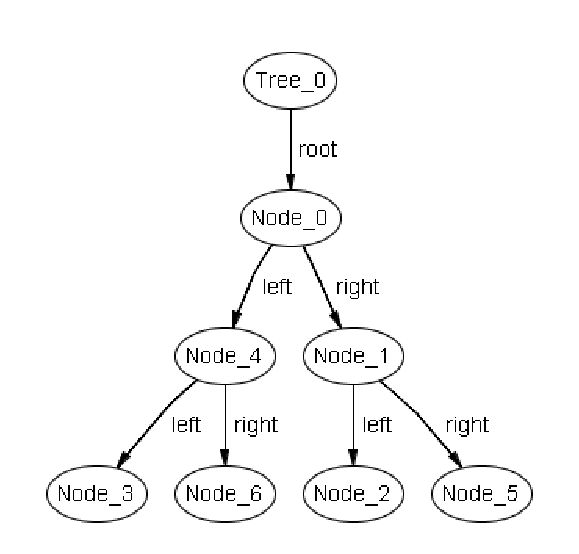
\includegraphics[scale=0.65]{Figures/correct_pre.eps}}\label{fig:tree_correct_pre}
        %\subfigure[After correct deletion]{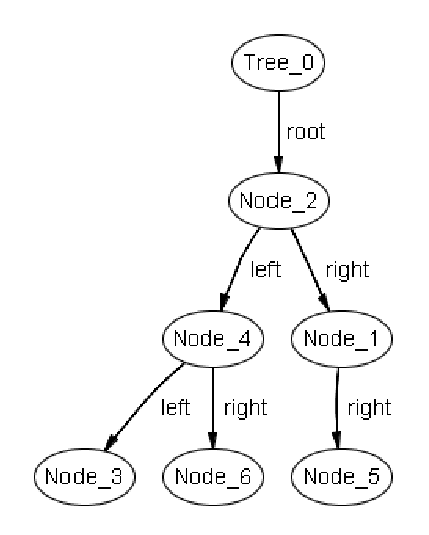
\includegraphics[scale=0.65]{Figures/correct_post.eps}}\label{fig:tree_correct_mainBody}
        \subfigure[Before deletion]{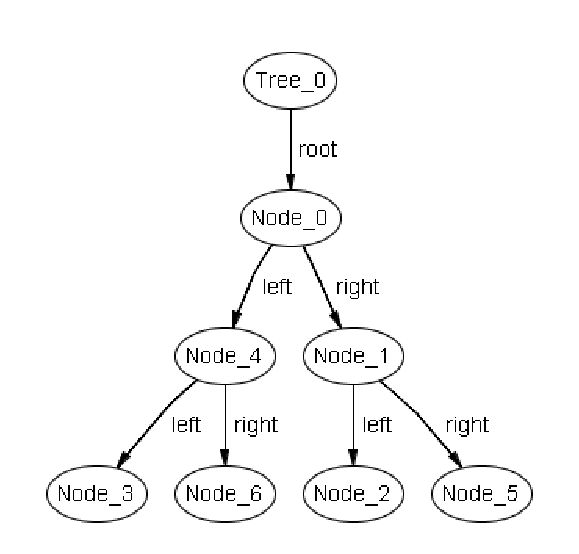
\includegraphics[scale=0.65]{Figures/correct_pre}}\label{fig:tree_correct_pre}
        \subfigure[After correct deletion]{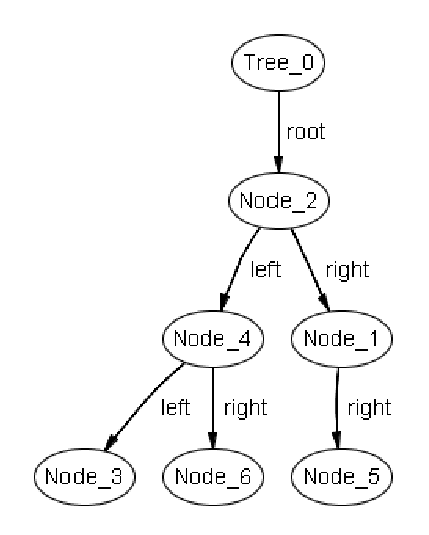
\includegraphics[scale=0.65]{Figures/correct_post}}\label{fig:tree_correct_mainBody}     
        }
    \caption[Visualization of tree]{Visualization of tree before and after correct deletion of the root node}
    \label{fig:tree_beforeAndAfter}
    \end{figure}

    \begin{singlespacing}
    \begin{figure}[H]
    \centering
    %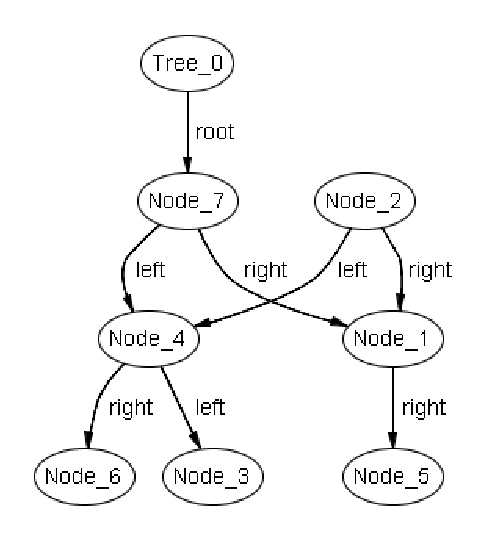
\includegraphics[scale=0.75]{Figures/commentedOutWithBetterNumber_post.eps}
    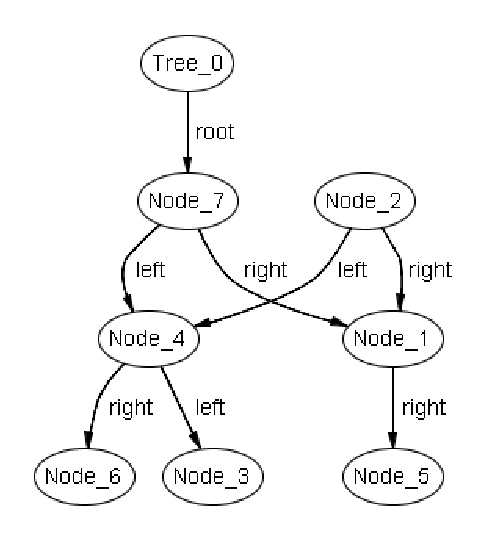
\includegraphics[scale=0.75]{Figures/commentedOutWithBetterNumber_post}
    \caption[Visualization of tree after deletion of root (error or omission)]{Visualization of tree
    after deletion of the root node, with an error of omission in the code.
    \texttt{Node\_7} represents the temporary node in the \texttt{swapNodes()} method.}
    \label{fig:tree_commentedOut_mainBody}
    \end{figure}
    \end{singlespacing}

\chapter{Embee: Implementation and Analysis}\label{ch:Embee2}


    \begin{singlespacing}
    \begin{Listing}[h]
    \fileinsmall{Examples/connectToVM.txt} \caption[Excerpt from
    \texttt{StateDumperThreads.java}]{Excerpt from \texttt{StateDumperThreads.java},
    showing how to connect to a second virtual machine executing the target code.  In
    this example, the target class is referenced by \texttt{javaClassName}.  The JPDA
    classes can be accessed by including the \texttt{tools.jar} archive in the program's
    classpath; this archive is found in the Java installation's \texttt{lib} directory}
    \label{list:connectToVM}
    \end{Listing}
    \end{singlespacing}


    \begin{figure}[h]
    \begin{singlespacing}
    \centering
        \subfigure[Specification of binary \texttt{next} relation]{
            \begin{minipage}{100pt}
                \filein{Examples/smallA.txt}
            \label{fig:smallBinary}
            \end{minipage}}
        \hspace{0.25in}
        \subfigure[Implementation of binary relation in (a)]{
            \begin{minipage}{100pt}
                \filein{Examples/smallB.txt}
            \label{fig:smallBinaryCode}
            \end{minipage}}
        \hspace{0.25in}
        \subfigure[Specification of ternary \texttt{next} relation]{
            \begin{minipage}{100pt}
                \filein{Examples/smallC.txt}
            \label{fig:smallTernary}
            \end{minipage}}
    \caption[Sample specification and implementation]{Sample specification and
    implementation of a binary relation; sample specification of a ternary relation}
    \end{singlespacing}
    \end{figure}

\section{Complexity and Performance}\label{sec:EmbeeComplexity}

\subsection{Definition of Terms}\label{sec:termDefn}

    The following terms...:

    \begin{Ventry}{\boldmath $\operatorname{arity}(r_i)$ \unboldmath}

        \boldmath \item[$scope$] \unboldmath
        The maximum number of objects...

        \boldmath \item[$R$] \unboldmath
        The number of relations...

        \boldmath \item[$r_i$] \unboldmath
        The $i^\text{th}$ relation in the specification, $1 \le i \le R$.

        \boldmath \item[$\operatorname{arity}(r_i)$] \unboldmath
        The arity of relation $r_i$...

        \boldmath \item[$N$] \unboldmath The total number...

        Given the calculated arities of a particular specification's relations, and the scope at
        a specific breakpoint, Equation~\ref{equation:N} can be used to determine $N$.
        \begin{equation}\label{equation:N}
        N = S \times scope + \sum_{i=1}^R scope ^ {arity(r_i)}
        \end{equation}

    \end{Ventry}



    The combined complexity of all four steps is
    \begin{equation*}
        O(N) + O(nN) + O(N^2) + O(F)
    \end{equation*}
    Again, these steps are completed once for every breakpoint in the target program's
    execution; therefore, the overall upper bound becomes
    \begin{equation*}
    \begin{split}
        & b \times O(N) + b \times O(nN) + b \times O(N^2) + b \times  O(F) \\
                   = ~ & O(bN + bnN + bN^2 + bF)
    \end{split}
    \end{equation*}


    The vector [$x_0$  $x_1$] represents the two possible atoms of type
    \texttt{X}.  With our naming scheme, $x_0$ represents \texttt{X\_0} and $x_1$
    represents \texttt{X\_1}.
    The binary relation itself is represented by a two-dimensional bit matrix where a 1 in
    position [$i$,$j$] means that there is a mapping between the $i^{th}$ atom of \texttt{X}
    and the $j^{th}$ atom of \texttt{Y}:

    \begin{gather*}
    \begin{bmatrix}
      r_{00} & r_{01} \\
      r_{10} & r_{11} \\
    \end{bmatrix} \quad
    \begin{bmatrix}
      \texttt{X\_0->Y\_0} & \texttt{X\_0->Y\_1} \\
      \texttt{X\_1->Y\_0} & \texttt{X\_1->Y\_1} \\
    \end{bmatrix}
    \end{gather*}
    \medskip

    Now, consider a fact stating that relation \texttt{r} is total, i.e.,

    \begin{center}
    \texttt{all x :~X | some y :~Y | x.r = y}
    \end{center}

    The CNF formula for our example fact, in scope~2, is
    \begin{equation*}
    \begin{split}
    & \neg(((x_0 \wedge r_{00}) \vee (x_1 \wedge r_{10})) \wedge \neg((x_0 \wedge r_{01})
    \vee (x_1 \wedge r_{11}))) \wedge \\ &\neg(\neg((x_0 \wedge r_{00}) \vee (x_1 \wedge
    r_{10})) \wedge ((x_0 \wedge r_{01}) \vee (x_1 \wedge r_{11})))
    \end{split}
    \end{equation*}
    \medskip

    Table~\vref{fig:fullRunTimesAllPhases} contains...

    \begin{singlespacing}
    \begin{center}
    \begin{threeparttable}
    \caption{Running times for each phase and total running time of Embee}
    \label{fig:fullRunTimesAllPhases}\begin{small}
        % Table generated by Excel2LaTeX from sheet 'Embee'
        \begin{tabular}{|l|c|c|c|c|c|c|c|} \hline

        \multicolumn{3}{|c|}{Test Case} & \multicolumn{ 5}{c|}{Running Time (m:ss)} \\ \hline

        \multicolumn{1}{|c|}{Object} & & Number of & & & \multicolumn{2}{c|}{ Phase 3} &  \\  \cline{6-7}

        \multicolumn{1}{|c|}{Model} & \raisebox{1.5ex}[0pt]{Scope} & Breakpoints &  \raisebox{1.5ex}[0pt]{Phase 1} & \raisebox{1.5ex}[0pt]{Phase 2} &   First 16 &   Last 4 &  \raisebox{1.5ex}[0pt]{Total} \\

        \hline
            List  &  20 &  20           &  0:07 &  0:32 &  0:12 &  06:39 & 07:30 \\
        \hline
            Graph &  20 &  19\tnote{a}  &  0:07 &  1:27 &  0:35 &  44:10 & 46:19 \\
        \hline
            Tree  &  20 &  20 &  0:04   &  1:20 &  0:21 &  06:04 &  07:49 \\
        \hline
        \end{tabular}
    \begin{tablenotes}
    \item[a] Breakpoints occur after the addition of each edge, i.e., the first
    breakpoint does not occur until the second node is added.
    \end{tablenotes}
        \end{small}
    \end{threeparttable}
    \end{center}
    \end{singlespacing}


    ...upper bound on Embee's performance:

    \begin{numcases}{\text{upper bound is}}
        O(bN^2) & if $scope \leq 16$ \notag \\
        O(bF)   & if $scope > 16$ \notag
    \end{numcases}



\chapter{Summary and Conclusions}\label{ch:Conclusion}

\section{Summary}

\section{Other Work}

\subsection{International Network for Social Network Analysis}

\section{Future Work}

\section{Conclusion}


%*************************************************************************************************************
% BIBLIOGRAPHY
%*************************************************************************************************************
% This GATHER command is useful for when you want to use WinEdt's Gather functionality, i.e., type
% \cite{} and a popup box appears with all of your citations to choose from.  Leave the % on the next line.
%GATHER{thesis.bib}

% Put in \nocite{*} so all entries in the bibliography are included
%\nocite{*}

\bibliographystyle{plain}
\bibliography{thesis}

%*************************************************************************************************************
% APPENDICES
%*************************************************************************************************************
\updatechaptername
%\appendixpage
\appendix

\chapter{Alloy Analyzer}\label{App:AnalyzerCode}

\section{Documentation}

\paragraph*{\large Package: \texttt{alloy.api}}

    %%%%%%%%%%%%%%%%%%%%%%%%%%%%%%%%%%%%%%%%%%%%%%%%%%%%%%%%%%%%
    % AlloyRunner
    %%%%%%%%%%%%%%%%%%%%%%%%%%%%%%%%%%%%%%%%%%%%%%%%%%%%%%%%%%%%
    \begin{singlespacing}
    \begin{center}
    \begin{tabularx}{\linewidth}{|l|X|} \hline
    \multicolumn{2}{|p{420pt}|}{\texttt{\large AlloyRunner}} \\ \hline \hline

    \multicolumn{2}{|p{420pt}|}{\small This class provides...} \\
    \multicolumn{2}{|p{420pt}|}{} \\
    \multicolumn{2}{|p{420pt}|}{\small To do an analysis...}\\ \hline \hline

    {\small \texttt{analyzeCommand}} & {\small Run the actual...} \\ \hline

    {\small \texttt{prepareSpec}} & {\small Parse...} \\ \hline

    {\small \texttt{translateCommand}} & {\small Translate...} \\
    \hline

    \end{tabularx}
    \end{center}
    \end{singlespacing}

\chapter{Additional Analysis}\label{App:Analysis}

\section{Calculation of Arity}\label{AppSec:arity}


    Examples of arity calculations are shown in Table~\vref{table:arity}.  These calculations
    can be performed using either the equations listed in
    Figure~\vref{fig:arityEquations}...

   \begin{singlespacing}
    \begin{figure}[ht]
    \begin{boxedminipage}[h]{433pt}
        \begin{minipage}{400pt}

        Given:
            \begin{center}
            \begin{minipage}{350pt}
            $v$ is a variable of type \texttt{<var>}, i.e., an \texttt{id} (identifier)\\
            $m$ is a multiplicity expression of type \texttt{<multexpr> }\\
            $r$ is a relation of type \texttt{<relation>}, i.e., $r = v : m$ \\
            $e_1$, $e_2$, ... are expressions of type \texttt{<expr> }in $m$\\
            $x$ is an optional set multiplicity modifier of type \texttt{<setmult>}\\
            $y$, $z$ are optional relation multiplicity modifiers of type \texttt{<mult>}
            \end{minipage}
            \end{center}
        The arity equations are:
        \end{minipage}
        \begin{equation}
        \operatorname{arity}(r) = 1 + \operatorname{arity}(m) \text{,~~where $r$ is of the form $v : m$}
        \label{equation:arity1}
        \end{equation}
        \begin{subequations}
        \begin{numcases}{arity(m)=}
            1 & if $m$ is of the form $x~v$ \label{equation:arity2a} \\
            arity(e_1) + arity(e_2) & if $m$ is of the form $e_1 ~y$ \texttt{->} $z~ e_2$ \label{equation:arity2b}
        \end{numcases}
        \end{subequations}
        \begin{subequations}
        \begin{numcases}{arity(e)=}
            1 & if $e$ is of the form \texttt{id} \label{equation:arity3a} \\
            arity(e_1) & if $e$ is of the form $(e_1)$ \label{equation:arity3b} \\
            arity(e_1) + arity(e_2) & if $e$ is of the form $e_1$ \texttt{->} $e_2$ \label{equation:arity3c}
        \end{numcases}
        \end{subequations}
        \label{equation:arityEquations}
    \end{boxedminipage}
    \caption{Equations to compute arity of relations} \label{fig:arityEquations}
    \end{figure}
    \end{singlespacing}

        \begin{singlespacing}
        \begin{table}[H]
        \begin{center}
        \caption{Example arity calculations}\label{table:arity}
        \bigskip
        \begin{tabular}{|l|c|c|}\hline
        \multicolumn{1}{|c|}{relation $r_i$} & \multicolumn{1}{c|}{$arity(r_i)$} & \multicolumn{1}{c|}{arity equations used} \\ \hline
        \verb|f : A |                    & 2 & \eqref{equation:arity1}, \eqref{equation:arity2a} \\ \hline
        \verb|f : option A|              & 2 & \eqref{equation:arity1}, \eqref{equation:arity2a} \\ \hline
        \verb|f : A -> A|                & 3 & \eqref{equation:arity1}, \eqref{equation:arity2b}, \eqref{equation:arity3a} \\ \hline
        \verb|f : A -> ? B|              & 3 & \eqref{equation:arity1}, \eqref{equation:arity2b}, \eqref{equation:arity3a} \\ \hline
        \verb|f : A -> B -> C|           & 4 & \eqref{equation:arity1}, \eqref{equation:arity2b}, \eqref{equation:arity3c}, \eqref{equation:arity3a} \\ \hline
        \verb|f : A -> B ? -> ! C|       & 4 & \eqref{equation:arity1}, \eqref{equation:arity2b}, \eqref{equation:arity3a}, \eqref{equation:arity3c} \\ \hline
        \verb|f : A -> B -> C -> D|      & 5 & \eqref{equation:arity1}, \eqref{equation:arity2b}, \eqref{equation:arity3c}, \eqref{equation:arity3a} \\ \hline
        \end{tabular}
        \end{center}
        \end{table}
        \end{singlespacing}

\section{Comparison of $N$}\label{AppSec:CompareN}



\subsection{Reasoning about $N$ in terms of $n$}\label{AppSec:Nandn}

    It is possible to determine an upper bound on the size of $N$, relative to the size
    of $n$.  To do this, we re-examine Equation~\ref{equation:N}.

    From Equation~\ref{equation:N}, we have:
    \begin{equation*}
        N = S \times scope + \sum_{i=1}^R scope ^ {arity(r_i)}
    \end{equation*}

    In the worst-case, the scope is equal to the total number of objects that exist at a
    particular breakpoint, i.e., $scope = n$.
    \begin{equation*}
        N = S n + \sum_{i=1}^R n ^ {arity(r_i)}
    \end{equation*}

    We can expand the summation to
    \begin{equation*}
        N = S n + n^{arity(r_1)} + n^{arity(r_2)} + ... + n^{arity(r_R)}
    \end{equation*}

    Because...
    \begin{equation*}
        O(N) = O(S n) + O(n^{arity(r_1)}) + O(n^{arity(r_2)}) + ... +
        O(n^{arity(r_R)})
    \end{equation*}

    We assume that all $R$ relations in the specification have the same arity, and that this
    arity is represented by a value $x \geq 2$.  Therefore...
    \begin{align}
        O(N) & = O(S n) + R \times O(n^x) \notag \\
             & = O(S n) + O(R n^x)
        \label{equation:NwithSR}
    \end{align}

    Equation~\ref{equation:NwithSR} demonstrates...

    Because both $S$ and $R$ are finite numbers, it is possible to further reduce
    Equation~\ref{equation:NwithSR} to
    \begin{align}
        O(N) & = O(n) + O(n^x) \notag \\
             & = O(n^x)
        \label{equation:NwithoutSR}
    \end{align}

    Therefore...





\clearpage
\section{Estimation of $F$}\label{AppSec:F}

    For example, Table~\vref{table:numOperators} contains the values of $F$...

    \begin{singlespacing}
    \begin{table}[H]
    \caption[Estimate of Boolean formula size]{Estimate of Boolean formula size,
    determined by number of Boolean operators (``and", ``or", ``not")}
    \label{table:numOperators}
        \begin{center}

        \bigskip

        % Table generated by Excel2LaTeX from sheet 'formula (extract)'
        \begin{tabular}{|c|r|r|r|r|}
        \hline
            \multicolumn{ 5}{|c|}{\textbf{Example 1 - List}} \\
        \hline
            $scope$ & \multicolumn{1}{c|}{$N$} & \multicolumn{1}{c|}{0 Facts} & \multicolumn{1}{c|}{1 Fact} & \multicolumn{1}{c|}{2 Facts} \\
        \hline
                1 &  4 &    23  &     34  &     43  \\
                2 & 12 &   197  &    657  &    729  \\
                3 & 24 &   671  & 13,799  & 15,200  \\
                4 & 40 & 1,731  & 91,435  & 96,771  \\
        \hline
        \end{tabular}

        \bigskip

        % Table generated by Excel2LaTeX from sheet 'formula (extract)'
        \begin{tabular}{|c|r|r|r|r|r|}
        \hline
            \multicolumn{ 6}{|c|}{\textbf{Example 2 - Graph}} \\
        \hline
            $scope$ & \multicolumn{1}{c|}{$N$} & \multicolumn{1}{c|}{Facts} & \multicolumn{1}{c|}{1 Fact} & \multicolumn{1}{c|}{2 Facts} & \multicolumn{1}{c|}{3 Facts} \\
        \hline
                1 & ---&   ---  &     ---  &       ---  &       ---  \\
                2 & 16 &   185  &   1,005  &     1,783  &     2,181  \\
                3 & 42 &   674  &  66,722  &   118,250  &   142,328  \\
                4 & 88 & 1,787  & 635,811  & 1,153,063  & 1,319,611  \\
        \hline
        \end{tabular}

        \bigskip

        % Table generated by Excel2LaTeX from sheet 'formula (extract)'
        \begin{tabular}{|c|r|r|r|r|r|r|}
        \hline
            \multicolumn{ 7}{|c|}{\textbf{Example 3 - Tree}} \\
        \hline
            $scope$ & \multicolumn{1}{c|}{$N$} & \multicolumn{1}{c|}{0 Facts} & \multicolumn{1}{c|}{1 Fact} & \multicolumn{1}{c|}{2 Facts} & \multicolumn{1}{c|}{3 Facts} & \multicolumn{1}{c|}{4 Facts} \\
        \hline
                1 &  7 &    39  &      78  &      93  &     103  &     104  \\
                2 & 22 &   367  &   1,601  &   2,487  &   2,629  &   2,715  \\
                3 & 45 & 1,283  &  38,528  &  73,472  &  76,196  &  76,568  \\
                4 & 76 & 3,359  & 234,595  & 456,459  & 466,979  & 468,087  \\
        \hline
        \end{tabular}
        \end{center}
    \end{table}
    \end{singlespacing}


\clearpage
\subsection{Test Series}

    Table~\vref{table:tests} summarizes...

    \begin{singlespacing}
    \begin{table}[H]
    \begin{center}
    \caption{Test series for evaluating the running time of conformance checking}
    \begin{tabular}{|c|c|c|c|c|c|c|c|c|} \hline
      % after \\: \hline or \cline{col1-col2} \cline{col3-col4} ...
      Series &  &  &  &  & Number &  &  & Number \\
      Name &
      \raisebox{1.5ex}[0cm][0cm]{Example} &
      \raisebox{1.5ex}[0cm][0cm]{$S$} &
      \raisebox{1.5ex}[0cm][0cm]{$R$} &
      \raisebox{1.5ex}[0cm][0cm]{$\operatorname{arity}(r_i)$} &
      of Facts &
      \raisebox{1.5ex}[0cm][0cm]{$scope=n$} &
      \raisebox{1.5ex}[0cm][0cm]{$N$} &
      of Tests \\ \hline

      E1F0 & 1            & 2 & 2 & 2, 2        & 0 & 1,2,...,40 & 4 - 3,280   & 40 \\ \cline{1-1} \cline{6-9}
      E1F1 & \emph{List}  &   &   &             & 1 & 1,2,...,32 & 4 - 1,984   & 32 \\ \cline{1-1} \cline{6-9}
      E1F2 &              &   &   &             & 2 & 1,2,...,31 & 4 - 1,984   & 31 \\ \hline
      E2F0 & 2            & 2 & 2 & 2, 3        & 0 & 2,3,...,40 & 16 - 65,680 & 39 \\ \cline{1-1} \cline{6-9}
      E2F1 & \emph{Graph} &   &   &             & 1 & 2,3,...,40 & 16 - 33,856 & 39 \\ \cline{1-1}\cline{6-9}
      E2F2 &              &   &   &             & 2 & 2,3,...,34 & 16 - 33,856 & 33 \\ \cline{1-1}\cline{6-9}
      E2F3 &              &   &   &             & 3 & 2,3,...,24 & 16 - 14,448 & 23 \\ \hline
      E3F0 & 2            & 3 & 4 & 2, 2, 2, 2  & 0 & 1,2,...,40 & 7 - 6,520   & 40 \\ \cline{1-1} \cline{6-9}
      E3F1 & \emph{Tree}  &   &   &             & 1 & 1,2,...,40 & 7 - 6,520   & 40 \\ \cline{1-1}\cline{6-9}
      E3F2 &              &   &   &             & 2 & 1,2,...,32 & 7 - 4,192   & 32 \\ \cline{1-1}\cline{6-9}
      E3F3 &              &   &   &             & 3 & 1,2,...,32 & 7 - 4,192   & 32 \\ \cline{1-1}\cline{6-9}
      E3F4 &              &   &   &             & 4 & 1,2,...,32 & 7 - 4,192   & 32 \\ \hline
      \multicolumn{8}{|r|}{Total Number of Tests (Conformance Checks)} & 412 \\ \hline
    \end{tabular}
    \label{table:tests}
    \end{center}
    \end{table}
    \end{singlespacing}

%\addappheadtotoc

%*************************************************************************************************************
% GLOSSARY
% Using a glossary is more than beginners need to know; leaving the packages, etc. here for now.
%*************************************************************************************************************
%\usepackage[nonumberlist]{glossaries}
%\usepackage[refpages]{gloss}  % for my glossary
                              % refpages shows the first page where the term occurs
%-------------------------------------------------------------------------------------------------------------
% Tell Latex to make a glossary
%*************************************************************************************************************
%\makeglossaries  % tell latex to make the glossary
%\glossarystyle{list}

%*************************************************************************************************************
% INDEX
%*************************************************************************************************************
% Here's where the index would be printed, if you created one.  Remove the % on the next line.
%\printindex


%*************************************************************************************************************
\end{document}
